\newpage
%%%%%%%%%%%%%%%%%%%%%%%%%%%%%%%%%%%%%%%%%%%%%%%%%%%%%%%%%%%%%%%%
%%%%%%%%%%%%%%%%%%%%%%%%%%%%%%%%%%%%%%%%%%%%%%%%%%%%%%%%%%%%%%%%
%%%%%%%%%%%%%%%%%%%%%%%%%% Enunciado %%%%%%%%%%%%%%%%%%%%%%%%%%%

\begin{myblock}
\phantomsection\addcontentsline{toc}{section}{Ejercicio \#10 | Descripción del corpus}
\section*{Ejercicio \#10 | Descripción del corpus}

Se ha realizado un análisis sobre el valor terapéutico del ácido ascórbico (Vitamina C) en relación
a su efecto sobre la gripe común. Se tiene una tabla $2 \times 2$ con los recuentos
correspondientes para una muestra de 279 personas.

Aplica un modelo lineal para determinar si existe ecvidencia suficiente para asgurar que el ácido 
ascorbico ayuda a tener menos gripe. 

\end{myblock}

%%%%%%%%%%%%%%%%%%%%%%%%%%%%%%%%%%%%%%%%%%%%%%%%%%%%%%%%%%%%%%%%
%%%%%%%%%%%%%%%%%%%%%%%%%%%%%%%%%%%%%%%%%%%%%%%%%%%%%%%%%%%%%%%%

\begin{table}[h!]
\centering
\caption{Tabla de contingencia del estudio sobre el Ácido Ascórbico.}
\label{tab:gripe}
\begin{tabular}{l|cc|c}
\multicolumn{1}{c}{} & \textbf{Gripe} & \textbf{No Gripe} & \textit{Totales} \\
\hline
Placebo             & 31 & 109 & 140 \\
Acido Asc\'{o}rbico & 17 & 122 & 139 \\
\hline
\textit{Totales}    & 48 & 231 & 279 \\
\end{tabular}
\end{table}

%%%%%%%%%%%%%%%%%%%%%%%%%%%%%%%%%%%%%%%%%%%%%%%%%%%%%%%%%%%%%%%%
%%%%%%%%%%%%%%%%%%%%%%%%%%%%%%%%%%%%%%%%%%%%%%%%%%%%%%%%%%%%%%%%

\begin{figure}[h!]
    \centering
    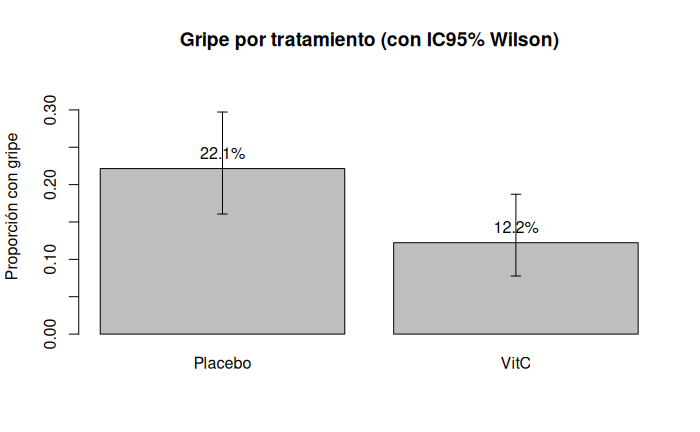
\includegraphics[width=0.7\linewidth]{Images/gripe-p10.png}
    \caption{Gripe GLM.}
    \label{fig:gripe-10}
\end{figure}


Se evaluó el efecto terapéutico del ácido ascórbico (Vitamina C) sobre la incidencia de gripe en un ensayo con $n=279$ personas, asignadas a los grupos de Placebo ($n=140$) y Vitamina C ($n=139$). La respuesta considerada fue binaria: presencia o ausencia de gripe. La tabla de contingencia observada fue: Placebo con 31 casos de gripe y 109 sin gripe, y Vitamina C con 17 casos de gripe y 122 sin gripe. En total se observaron 48 casos de gripe y 231 individuos sanos.

Para el análisis se ajustó un modelo lineal generalizado binomial con enlace logit de la forma
\[
\log \frac{\Pr(Y=1 \mid T)}{1 - \Pr(Y=1 \mid T)} = \beta_0 + \beta_1 \,\mathbb{1}\{T=\text{VitC}\},
\]
donde $Y$ indica la ocurrencia de gripe y $T$ el tratamiento recibido. El interés radica en contrastar la hipótesis unilateral de que $\beta_1 < 0$, es decir, que la administración de Vitamina C reduce la probabilidad de presentar gripe en comparación con el placebo. 

Los resultados del modelo muestran un intercepto estimado de $\hat\beta_0=-1.257$ (SE=0.204), correspondiente al log-odds de gripe en el grupo Placebo, y un coeficiente de tratamiento $\hat\beta_1=-0.713$ (SE=0.329). La odds ratio estimada de Vitamina C respecto a Placebo es $\widehat{\text{OR}}=\exp(\hat\beta_1)=0.490$, con un intervalo de confianza del 95\% dado por $[0.257,\,0.934]$. Esto indica que las odds de gripe con Vitamina C son aproximadamente 51\% menores que con Placebo. La prueba de Wald bilateral produce un valor-$p=0.030$, mientras que en la dirección unilateral favorable a Vitamina C se obtiene $p=0.015$, lo que proporciona evidencia a favor del efecto protector.

Se aplicaron pruebas adicionales de independencia para verificar la robustez del resultado. La prueba de $\chi^2$ de Pearson entrega un estadístico $X^2=4.81$ con un valor-$p=0.028$, lo cual sugiere asociación entre el tratamiento y la incidencia de gripe. Por su parte, la prueba exacta de Fisher unilateral, especificando la hipótesis de que Placebo presenta mayor odds de gripe que Vitamina C, arroja un valor-$p=0.0205$ y un intervalo de confianza unilat. al 95\% de $[1.13,\,\infty)$ para la odds ratio en la escala Placebo vs Vitamina C, equivalente a concluir que la odds ratio Vitamina C vs Placebo es menor que 1. Así, las tres pruebas son consistentes en apoyar la hipótesis de interés.

En términos de riesgos absolutos, la proporción de gripe en el grupo Placebo fue de $\hat p_{\text{Placebo}}=31/140=0.221$, mientras que en el grupo Vitamina C fue de $\hat p_{\text{VitC}}=17/139=0.122$. La reducción absoluta del riesgo estimada es $\hat p_{\text{VitC}} - \hat p_{\text{Placebo}} = -0.099$, es decir, una disminución de 9.9 puntos porcentuales. El riesgo relativo estimado es $\widehat{\text{RR}} = 0.552$, lo cual implica que el riesgo de gripe con Vitamina C es aproximadamente 45\% menor que con Placebo. Finalmente, el número necesario a tratar (NNT) se aproxima como $1/0.099 \approx 10$, interpretándose que, bajo condiciones similares, se deberían tratar 10 personas con Vitamina C para evitar un caso adicional de gripe.

En conclusión, la evidencia estadística proveniente del modelo logístico, la prueba de Pearson y la prueba exacta de Fisher unilateral apoya de manera consistente que el ácido ascórbico reduce la incidencia de gripe en comparación con placebo. La magnitud del efecto es clínicamente relevante, con un odds ratio estimado de 0.49, un riesgo relativo de 0.55, una reducción absoluta del riesgo cercana al 10\% y un número necesario a tratar de alrededor de 10. Estos resultados constituyen un respaldo empírico a la hipótesis de que la Vitamina C ejerce un efecto protector frente a la gripe común.

\clearpage